\chapter{Цилиндрическая поверхность.}

\begin{definition}[\textbf{Цилиндрическая поверхность.}]
	Поверхность Cyl называется {\color{Black} \textbf{цилиндрической}}, если она образована параллельным перемещением некоторой прямой $l$, называемой {\color{Black} \textbf{образующей}}, вдоль некоторой кривой $\gamma$, называемой {\color{Black} \textbf{направляющей}}.
\end{definition}

\begin{conseq}
	Векторы, перпендикулярные каждой точке цилиндрической поверхности ({\color{Black} \textbf{нормали поверхности}}), лежат в одной плоскости.
\end{conseq}

\begin{definition}
	$S^1 = \{ x \in \mathbb{R}^3: \; |x| = 1 \}$.
\end{definition}

\begin{conseq}
	Единичные нормали цилиндрической поверхности, выпущенные из $\vec{0}$, лежат на $C$. $C$ -- сечение $S^1$ некоторой плоскостью $\Pi$ через $\vec{0}$: $C_{big} = S^1 \cap \Pi$

	\vspace{1cm}
	\begin{figure}[h!]
	\center{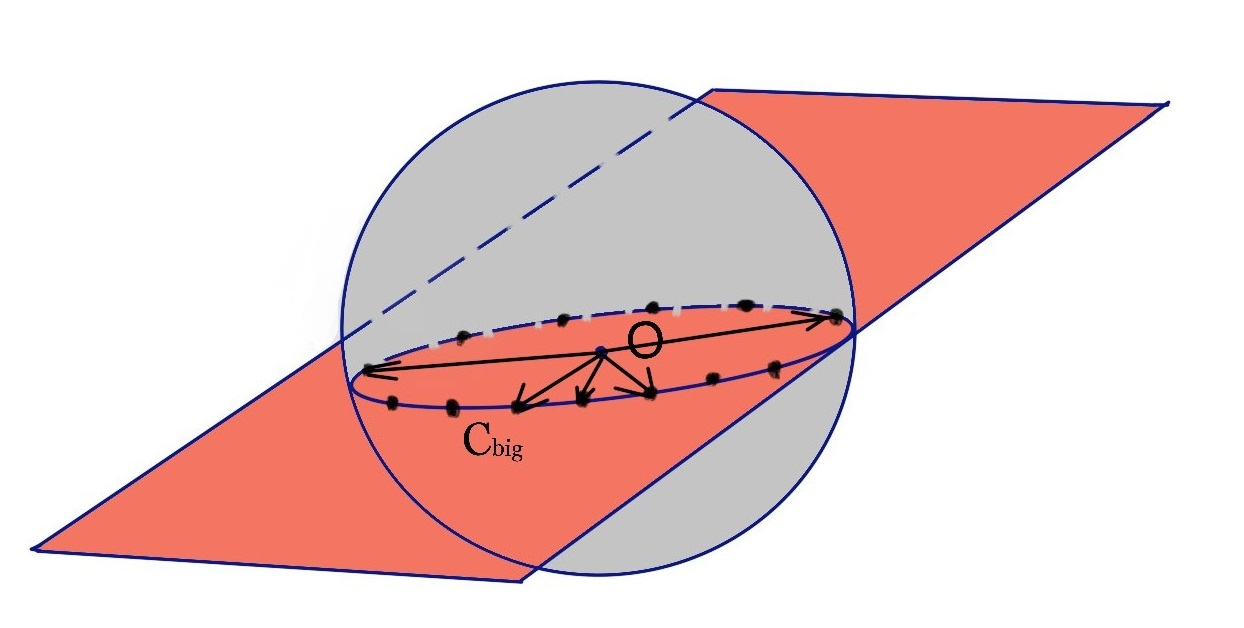
\includegraphics[scale=0.4]{1.jpg}}
	\end{figure}\vspace{0.5cm}
\end{conseq} \newpage

Рассмотрим множество единичных нормалей $\{ n_j \}_{j = 1}^N$ граней исходного многогранника P, выпущенных из $\vec{0}.$ 
Тогда для нахождения цилиндрических поверхностей на многограннике будем искать множества $N^{(i)} = \{ n_j \}_{j \in T_i}$, лежащие на C, где $T_i \subset \{ 1, \ldots, N\}$ -- набор индексов. Найденные наборы граней, соответствующие $N^{(i)}$, обозначим $\{ R_i\}$.

\begin{remark}
	$\vec{0}, \; N^{(j)}$ лежат на окружности C с некоторой погрешностью.
\end{remark}

